\chapter{Gestión y Planificación del proyecto}
En este capítulo se tratarán todas las cuestiones relacionadas con la gestión del proyecto: la metodología de desarrollo escogida, la gestión del alcance, tiempo, riesgos y costes.

Lo que se busca con ello es determinar claramente los objetivos a cumplir durante la realización, así como asegurar el buen avance del proyecto repartiendo de forma adecuada los recursos, previniendo posibles problemas y estableciendo un marco de trabajo para estructurar, planificar y controlar el desarrollo del software.

\section{Gestión del alcance}
En esta sección se determinará el alcance general del proyecto, así como los criterios que serán necesarios para la aceptación de éste, y las restricciones a las que está sometido. Por último, se detallarán los entregables que se generarán al finalizar.

\subsection{Descripción del alcance del proyecto}
Para la creación de acertijos por parte de los usuarios y la posibilidad de que la comunidad de usuarios de la aplicación disponga de la posibilidad de poder resolver éstos e interactuar, es necesario tener en cuenta una serie de factores:

\begin{itemize}
    \item \textbf{Por parte de los usuarios:}
    \begin{itemize}
        \item \textbf{Datos personales del usuario:} será necesario almacenar datos personales tales como nombre y apellidos, contraseña y \textit{nick} o nombre de usuario.
        \item \textbf{Acertijos escritos:} es muy importante asociar cada usuario con el acertijo que él mismo ha escrito.
        \item \textbf{Propuestas de solución a acertijos:} también muy importante el registro en el sistema de las posibles propuestas de un usuario para la solución de los acertijos.
        \item \textbf{Valoración de las propuestas de solución a los acertijos del usuario:} un usuario podrá acceder a las soluciones propuestas para sus acertijos y puntuar según lo cerca que se encuentren de la solución final.
    \end{itemize}
    \item \textbf{Por parte de los acertijos:}
    \begin{itemize}
        \item \textbf{Datos específicos de cada acertijo:} será necesario almacenar el título, el acertijo, la solución al mismo, 3 pistas para facilitar el comienzo a los otros usuarios la búsqueda de la solución y el estado del porcentaje de resolución de la misma.
        \item \textbf{Acertijos escritos:} es muy importante asociar cada acertijo con el usuario que lo ha escrito.
        \item \textbf{Soluciones propuestas de cada acertijo:} también muy importante el registro en el sistema de las propuestas para la solución de cada acertijo.
    \end{itemize}
\end{itemize}

La aplicación contendrá dos funcionalidades principales, destacadas y que sustentarán el objetivo principal del proyecto: escritura de acertijos y resolución de los mismos.

Para la funcionalidad de escritura, el sistema será el encargado de almacenar los acertijos propuestos y mostrarlos al mundo. En la segunda funcionalidad nombrada, será el propio sistema el encargado de gestionar la interacción entre usuarios con el objetivo de resolver los enigmas.

\subsection{Criterios de aceptación}
El proyecto será aceptado si la aplicación será capaz de permitir a un usuario la escritura de un acertijo completo. Además, se podrá permitir al usuario proponer soluciones a distintos acertijos propuestos por otros usuarios. 

Por último, un usuario será capaz de poder evaluar las propuestas de solución de cada uno de sus acertijos y, éstos, automáticamente actualizarán su estado de resolución basándose en las puntuaciones de las mismas.
\subsection{Restricciones del proyecto}
El proyecto debe suponer un total de 12 créditos, es decir, unas 300 horas de trabajo, y debe ser entregado no más tarde del 07/09/2018.

\subsection{Entregables del proyecto}
Como resultado del proyecto se considerarán los siguientes entregables:
\begin{itemize}
    \item Código fuente de todo el software desarrollado\cite{proyectogithub}.
    \item Memoria del trabajo de fin de grado\cite{memoriagithub}.
\end{itemize}

\section{Metodología de desarrollo}
Antes de iniciar cualquier proyecto de desarrollo de software, es muy importante determinar y definir qué metodología se seguirá. El objetivo es establecer un plan de acción, reduciendo así el riesgo de que se sufran retrasos en el desarrollo, sobre costes, o un mal planteamiento que suponga el fracaso del proyecto en su totalidad. Probablemente en la práctica existan tantas metodologías de trabajo como proyectos de desarrollo, pero en todos los casos es necesario tener en cuenta las características y particularidades del proyecto a la hora de elegir y adaptar una metodología concreta al caso específico.

En el caso concreto de este proyecto, nos encontramos con varios factores importantes que resultan determinantes para la elección de una metodología concreta:

\begin{itemize}
    \item Al tratarse de una aplicación que necesita de interfaz, es necesario dedicar tiempo al desarrollo de la misma de una manera independiente a las demás partes. 
    \item En esta aplicación será necesaria la creación de una base de datos donde almacenar todos los acertijos, usuarios y propuestas de solución.
    \item Al tener que desarrollar una API REST que gestione las peticiones desde la interfaz y la base de datos, será necesario dedicar tiempo para el desarrollo de la misma, no de manera independiente, pues se necesita previamente una conexión de ésta con la base de datos.
\end{itemize}

Por ello, como metodología de desarrollo para mi proyecto lo mejor es crear una mezcla entre la metodología/\textit{framework} SCRUM y la filosofía/práctica DevOps.

El lado SCRUM aporta la creación de un marco de desarrollo de software con el que se obtiene un mayor control y flexibilidad a la hora de enfrentar la incertidumbre, los cambios y los riesgos. Este marco permite realizar modificaciones a la planificación y requisitos de forma controlada y rápida, evitando así que el proyecto fracase por no realizarlos a tiempo. Además, permite que el contacto con el cliente sea mayor y continuo, evitando así que exista demasiada incertidumbre.

Con la cultura DevOps se extrae la idea del desarrollo basado en pruebas \cite{desarrollotests}\cite{desarrollotests2}. Con esto se obtiene que para cada entregable existe la garantía de que es un producto de calidad, pues ha pasado previamente todos los tests que describían su funcionalidad.

\subsection{SCRUM}

Las metodologías ágiles\cite{scrum} surgen como respuesta a los problemas característicos de las metodologías tradicionales. Tanto SCRUM como otras metodologías ágiles (Iconix, Cristal Methods), se basan en los siguientes principios:

\begin{itemize}
    \item Es más importante que se desarrolle un producto de software de calidad y que funcione que escribir una documentación exhaustiva. 
    \item Las interacciones entre individuos son más importantes que las herramientas y procesos utilizados.
    \item La comunicación con el cliente es vital para el éxito del proyecto.
    \item Aún cuando establecer un plan es necesario, es más importante el contar con una buena capacidad de respuesta ante los cambios.
\end{itemize}

\subsubsection{Características de SCRUM}
Esta metodología se centra en el desarrollo incremental iterativo. A cada una de estas iteraciones las llamaremos \textbf{\textit{Sprint}}, y normalmente serán de una duración corta entre 3 y 4 semanas. Cada \textit{sprint} termina con una pieza clave de software completa y funcional.

Se prioriza el trabajo que resulta más valioso para el desarrollo del proyecto, con el objetivo de maximizar la utilidad de lo que se desarrolla. Los requisitos y la prioridad de éstos se revisan regularmente, normalmente al inicio de cada \textit{sprint}. El objetivo es construir de forma incremental un producto que se ajuste realmente a las necesidades del cliente, asegurando así su satisfacción.

Para mantener el ritmo de trabajo, sometido a constantes cambios, es necesario que el equipo se centre en construir \textbf{software de calidad}, pero para que esto pueda ser posible son necesarios dos aspectos: la gestión del proyecto debe asegurar una buena definición de las características deseables y evitar cualquier obstáculo que pueda afectar el trabajo del equipo; además el cliente debe entusiasmarse realmente por el proyecto desarrollado, de forma que exista un compromiso real que se mantenga tras la finalización de cada \textit{sprint} con el objetivo de mantener la comunicación constantemente y conocer así sus necesidades reales.

\subsubsection{Herramientas y roles}
\textit{Sprint} define todas las funcionalidades requeridas del producto a desarrollar en el \textit{Product Backlog}, determinando su prioridad, valor y riesgo, además de una estimación (de forma muy general) de la cantidad de trabajo que supone desarrollarla. Esta lista evoluciona a lo largo de todo el desarrollo.
		
		Además esta metodología define tres roles: el \textit{SCRUM master}, el \textit{Product owner} y el equipo de desarrollo.
			\begin{itemize}
				\item \textbf{\textit{SCRUM Master}}: es el líder del equipo. Se encarga de asegurarse de que se está siguiendo la metodología, se cumplen sus valores y prácticas. 
				\item \textbf{\textit{Product Owner}}: es el encargado de gestionar el desarrollo y el intermediario entre el cliente y el equipo. Se encarga de organizar y priorizar todas las funcionalidades requeridas.
				\item \textbf{Equipo de desarrollo}: es la pieza clave del proyecto. Puede estar a su vez subdividido en equipos de desarrollo, \textit{testing} y despliegue. 
			\end{itemize}
\subsubsection{Ciclo de trabajo}
	    SCRUM define un evento principal llamado Sprint, el cual corresponde con una ventana de trabajo que, tras su finalización, produce una versión funcional del producto. Dentro de cada \textit{sprint} tienen lugar una serie de eventos. La figura \ref{fig::cicloDeVidaSprint} muestra el ciclo de vida de un \textit{sprint}. 
	    
\begin{figure}
    \centerline{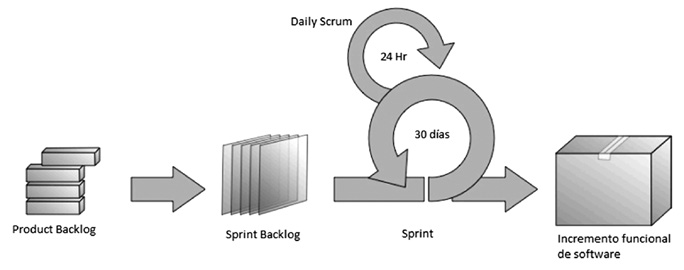
\includegraphics[width=11cm]{figuras/fasesDeUnSprint.png}}
    \caption{Ciclo de vida de un \textit{sprint}}
    \label{fig::cicloDeVidaSprint}
\end{figure}

\begin{enumerate}
		\item \textbf{Planificación de la iteración (\textit{Sprint planning})}: se define el plan de trabajo de este \textit{sprint} especifico determinando qué se entregara y cómo se logrará. Es decir, se determinan las funcionalidades a implementar y la estimación de cantidad de trabajo. Con todo esto, y partiendo de la información en el \emph{Product backlog}, se establece el \emph{Sprint backlog}.
		\item \textbf{Reunión diaria (\textit{Daily meeting})}: cada día se realiza una reunión para explicar los objetivos que se han alcanzado desde la ultima reunión y determinar qué se realizará el día siguiente. Esto permite identificar problemas rápidamente y evitar que se retrase el ritmo de trabajo. \item \textbf{Revisión de la iteración (\emph{Sprint review})}: se realiza tras la finalización del \textit{sprint} completo. Se revisa todo lo que se hizo y lo que no, se comentan los problemas que tuvieron lugar y cómo se resolvieron, y se revisan los resultados obtenidos. 
		\item \textbf{Retrospectiva de la iteración (\emph{Sprint retrospective})}: esta reunión tiene el objetivo de analizar los puntos a mejorar y los puntos fuertes del equipo con el fin de aumentar la productividad.
		\item \textbf{Replanificación}: conjuntamente con el cliente se revisa la planificación teniendo en cuenta los posibles cambios que hayan podido surgir durante el \emph{sprint}.
\end{enumerate}
			
\subsection{Aplicación de SCRUM a este proyecto}
Dado que la mayoría de las practicas de SCRUM están centradas en mejorar la productividad de un equipo, se han realizado una serie de adaptaciones teniendo en cuenta las características y circunstancias del proyecto. Se ha prescindido de la reunión diaria, pues el equipo de desarrollo está formado por una única persona. En este caso los \textit{sprints} tuvieron una duración de inicial de 3 semanas, por lo que en lugar del \textit{Daily meeting} se ha optado por realizar una autorreflexión semanal en la que se anotaba todo lo realizado hasta el momento y todas las actividades pendientes de abordar. Además, la reunión al final de cada \textit{sprint} se realizó con el tutor. Sin embargo, se mantuvo comunicación con éste constantemente a lo largo de todo el desarrollo.

\subsection{DevOps}

Las antiguas metodologías de desarrollo de software separaban en dos sectores bien diferenciados aquellos que escribían el software (Dpto. Desarrollo) de aquellos que desplegaban en la nube (Dpto. Sistemas) \cite{devops5}.

DevOps surge con la idea de romper esta división y unir en un solo equipo a aquellos que desarrollan software y aquellos que lo despliegan. Esta unión proporciona transparencia a la hora de consultar el estado del producto y las distintas etapas que ha superado o superará.

La filosofía DevOps se basa en los mismos principios que las metodologías ágiles. Sin embargo, con DevOps se quiere fomentar una cultura de equipo, en la que todas las personas que formen el equipo sepan qué está haciendo cada una.

\subsubsection{Características de DevOps}
Esta filosofía busca la calidad de un producto software, creado por un equipo que se adapte rápido a los cambios e inconvenientes que aparezcan a lo largo de su desarrollo. Estos cambios deben ser identificados con rapidez para su posterior solución.

DevOps engloba todas las buenas prácticas a tener en cuenta a la hora de la entrega, el desarrollo y la administración de aplicaciones a lo largo del ciclo de vida de desarrollo de software: \cite{devops7}

\begin{itemize}
    \item Desarrollo y revisión de código con la ayuda de un controlador de versiones.
    \item Uso de herramientas de integración continua
    \item Continuo \textit{testeo} del producto para obtener un software de calidad.
    \item Uso de un gestor de repositorio optimizar la descarga y el almacenamiento de archivos binarios utilizados y producidos en el desarrollo de software.
    \item Uso de un gestor que automatice el proceso de despliegue
    \item Uso de un gestor de aprovisionamiento que nos cargue las configuraciones que necesarias del proyecto.
    \item Monitorización del rendimiento de la aplicación.
\end{itemize}

\subsection{Aplicación de DevOps a este proyecto}

Para este proyecto se usará Git \footnote{https://git-scm.com/} como herramienta para el control de versiones y GitHub \footnote{https://github.com/} como servicio público donde almacenar el repositorio de la aplicación.

Es fundamental en este proyecto el desarrollo basado en pruebas y la integración continua en el repositorio. El código debe de estar testeado previamente antes de añadirlo oficialmente al repositorio del mismo si se quiere obtener un software de calidad.

En este proyecto el equipo está formado por una persona, por lo que el mismo equipo será transparente y formado por el sector de desarrollo y el sector de despliegue.


\subsection{Combinación de SCRUM y DevOps}

Como se ha explicado anteriormente, SCRUM nos define un marco para el desarrollo de la aplicación. Un marco donde se definen \textit{sprints} para la consecución de objetivos.

SCRUM se usará en este proyecto como una estructura que ayude a organizar y dividir los pasos para la creación de la aplicación, cada división la interpretaremos como un \textit{sprint}.

Dentro de cada \textit{sprint}, DevOps ayudará a la obtención de esos objetivos gracias a su filosofía basada en el uso de buenas prácticas relacionadas con el desarrollo basado en pruebas, herramientas de automatización para el despliegue y la revisión del código gracias a un controlador de versiones.

\section{Gestión de la configuración}
En esta sección se define la gestión de la configuración bajo la cual desarrollaremos todas las actividades que impliquen la creación, modificación o eliminación de alguno de los elementos de trabajo que conforman este proyecto, asegurando así que todo lo que concierne al proyecto sea válido durante la vida del mismo.

 Teniendo en cuenta que los elementos de trabajo de este proyecto son los ficheros de código fuente y todos los archivos que conforman la documentación, abordaremos esta sección especificando, de forma independiente, cómo se ha tratado cada tipo de elemento de trabajo.
 
\subsection{Gestión del código}

Para la gestión del código se creará un repositorio local con un  sistema de control de versiones, que a su vez se sincronizará con un repositorio remoto en GitHub, y por lo tanto almacenado en la nube. GitHub es un servicio web de control de versiones y desarrollo de software basado en Git\footnote{https://git-scm.com/}, publicado bajo una Licencia de código abierto. Esta copia remota previene el riesgo de pérdida del código fuente.

\subsection{Gestión de la documentación}
Para almacenar la documentación de este proyecto se utilizará un repositorio en GitHub llamado \textbf{Memoria\_TFG\_GuillermoMuriel} \footnote{https://github.com/guillesiesta/Memoria\_TFG\_GuillermoMuriel}.

Esta plataforma permite la creación de un repositorio cuyo lenguaje principal será LaTeX\footnote{https://www.latex-project.org/}, y le añade una licencia de código abierto.

En cuanto a la edición y gestión de la memoria del proyecto, se utilizará la plataforma online Overleaf v2\footnote{https://v2.overleaf.com/}. Dispone de control de versiones y edición en concurrencia. De la misma forma, al estar almacenada en la nube, se previene el riesgo de pérdida.

A la hora de realizar los diagramas de secuencia correspondientes, se ha utilizado la plataforma Plantuml\footnote{http://plantuml.com/}.

\section{Gestión del tiempo}
En este apartado se trata la planificación temporal del proyecto y las fases de la misma. Si bien se ha  establecido una planificación inicial, las tareas a realizar se especificarán de forma concreta a medida que se avance en el desarrollo del proyecto en función de los resultados obtenidos tras la finalización de cada \textit{sprint}.

\subsection{Planificación de los \textit{sprints}}

Teniendo en cuenta la metodología de desarrollo elegida, se ha optado por describir las tareas abordadas en cada \textit{sprint} y su correspondiente gráfico \textit{Burn-Down}. Los diagramas \textit{Burn-down} son gráficos de dos ejes que se utilizan para representar el avance ideal del proyecto frente al avance real. En el eje X se representa el tiempo y en el eje Y la cantidad de trabajo. Es necesario actualizarlo diariamente. Antes, procederemos a introducir una visión general de los requisitos temporales escogidos sobre la organización del tiempo:

Disponemos de 300 horas para la realización del proyecto.

Para la realización de este proyecto se van a programar 5 \textit{sprints} de 60 horas de duración cada uno. Por semana se trabajará de lunes a viernes unas 4 horas al día, en total 20 horas a la semana.

En total, se espera que cada \textit{sprint} dure 3 semanas .

Por lo que el proyecto, salvo imprevisto, debería estar finalizado en torno a las 15 semanas. 

Aproximadamente debería concluir en 4 meses.

\begin{figure}[hbtp]
\begin{subfigure}{.5\textwidth}
    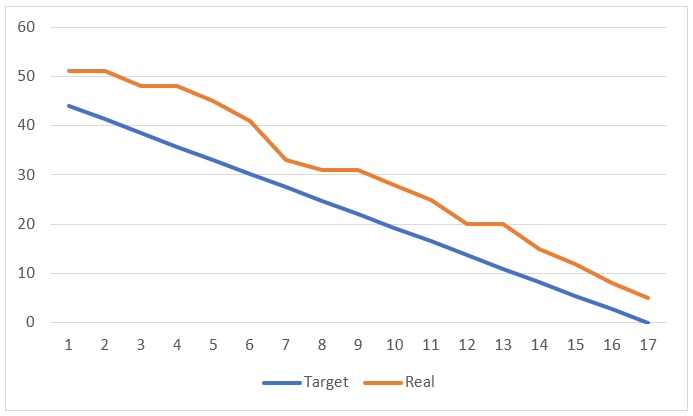
\includegraphics[width=\linewidth]{figuras/sprint1.png}
    \caption{\textit{Sprint} 1}
    \label{fig:sprint1}
\end{subfigure}
\begin{subfigure}{.5\textwidth}
    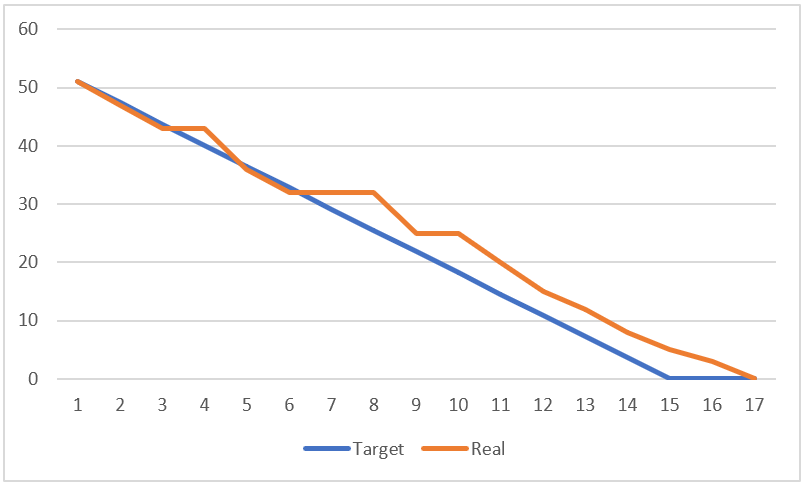
\includegraphics[width=\linewidth]{figuras/sprint2.png}
    \caption{\textit{Sprint} 2}
    \label{fig:sprint2}
\end{subfigure}
\begin{subfigure}{.5\textwidth}
    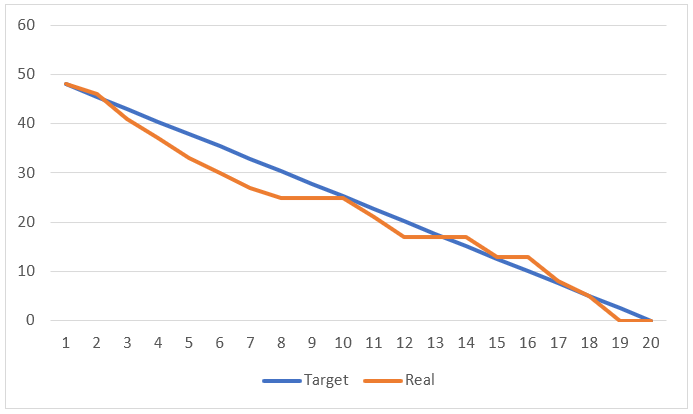
\includegraphics[width=\linewidth]{figuras/sprint3.png}
    \caption{\textit{Sprint} 3}
    \label{fig:sprint3}
\end{subfigure}
\begin{subfigure}{.5\textwidth}
    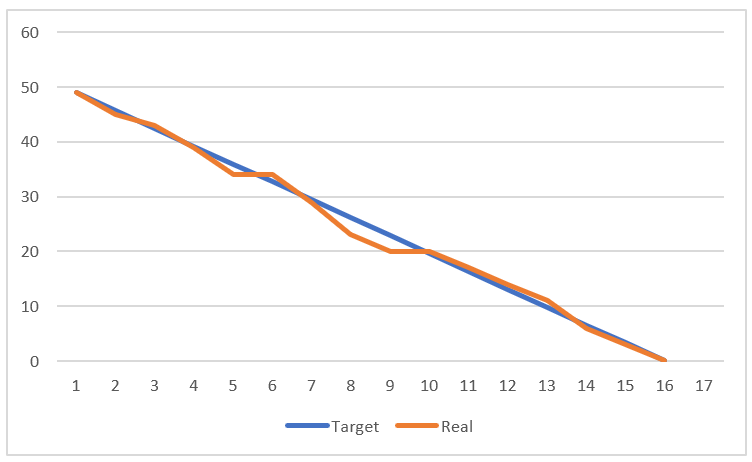
\includegraphics[width=\linewidth]{figuras/sprint4.png}
    \caption{\textit{Sprint} 4}
    \label{fig:sprint4}
\end{subfigure}
\begin{subfigure}{\textwidth}
    \centering
    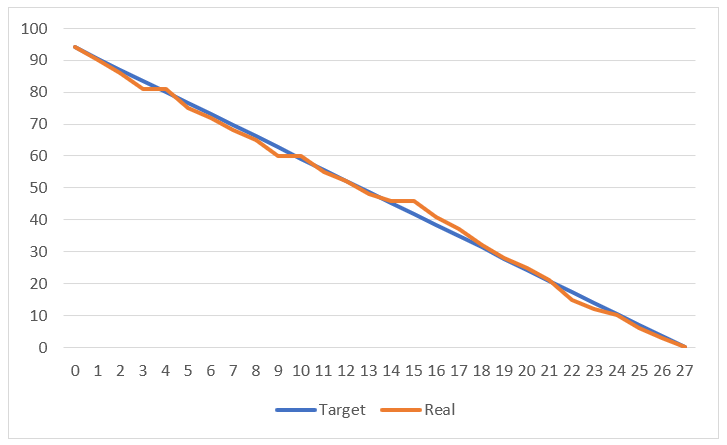
\includegraphics[width=.5\linewidth]{figuras/sprint5.png}
    \caption{\textit{Sprint} 5}
    \label{fig:sprint5}
\end{subfigure}
\caption{Gráficos \textit{burn-down} de los distintos \textit{sprints} del proyecto}
\label{fig:sprints}
\end{figure}

\begin{itemize}
    \item \textbf{\textit{Sprint} 1}. En esta primera fase determinará la organización temporal y se estudiará la viabilidad del proyecto. Se extraerán los requisitos y a partir de estos se hará un análisis de las tecnologías existentes para poder desarrollar el proyecto y desplegarlo en la nube y, se escogerán cuales serán las herramientas que más se adecúen a las necesidades del proyecto.
    
    \item \textbf{\textit{Sprint} 2}. En esta segunda fase se comenzará a trabajar en el almacenamiento de datos, se extraerá toda la documentación necesaria y se procederá a la construcción de la misma. La base de datos debe estar organizada, estructurada y desarrollada para que en el siguiente \textit{sprint} ya pueda ser utilizada.
    \item \textbf{\textit{Sprint} 3}. En este \textit{sprint} se procederá a construir el intermediario entre la interfaz y la base de datos. Lo llamaremos controlador, es decir, la API REST. Además, se implementaran tests que este controlador deberá de superar, así se confirma su correcto funcionamiento antes del montaje final. En esta fase conectaremos el controlador a la base de datos.
    \item \textbf{\textit{Sprint} 4}. Esta fase está desarrollada única y enteramente al desarrollo de la interfaz. Se escribirán los tests que deben de ser superados para que la interfaz sea apta para su despliegue.
    \item \textbf{\textit{Sprint} 5}. En la fase final se procederá a la unión de la interfaz y el controlador ya unido con la base de datos. A partir de aquí, con el sistema funcionando y testeado, procederemos a desplegarlo usando las tecnologías escogidas previamente. 
    
    Una vez la aplicación esté desplegada, se procederá a la redacción de la memoria.
\end{itemize}

\section{Gestión de riesgos}
Un riesgo de un proyecto es un evento o condición  que podría tener un efecto positivo o negativo sobre alguno de los recursos u objetivos del proyecto, como podría ser tiempo, coste, alcance o calidad. La gestión de riesgos es un proceso continuo que debe considerar tanto fuentes internas como externas de dichos riesgos. Por norma general, la materialización de un riesgo implica consecuencias negativas, por lo que la gestión de riesgos tiene un papel muy importante dentro de la gestión del proyecto. 

En esta sección se identificarán los posibles riesgos del proyecto, estimando la probabilidad de aparición y su impacto potencial. Posteriormente se definirán las estrategias y pasos a seguir para prevenirlos o minimizar su impacto en caso de que se materialicen.

\subsection{Identificación de riesgos}
\begin{itemize}
\item \textbf{R001} - No identificar correctamente los requisitos del proyecto.
\item \textbf{R002} - Dificultad en las tareas de formación.
\item \textbf{R003} - Aparición de nuevos requisitos.
\item \textbf{R004} - No conseguir ajustar la planificación a las horas requeridas.
\item \textbf{R005} - Cambios en la planificación o retrasos en la misma.
\item \textbf{R006} - Errores eligiendo las tecnologías para el desarrollo del proyecto.
\item \textbf{R007} - Disponibilidad del experto insuficiente.
\item \textbf{R008} - La estructura de los datos de partida cambia con el tiempo.
\item \textbf{R009} - Nulo o deficiente proceso de validación y verificación .
\item \textbf{R010} - Detección de fallos importantes en el software tras la validación.
\item \textbf{R011} - Detección de fallos importantes en la aplicación tras la validación.
\item \textbf{R012} - La interfaz no cumple con los requisitos.
\item \textbf{R013} - La API no cumple con los requisitos.
\item \textbf{R014} - La base de datos escogida no cumple con los requisitos.
\item \textbf{R015} - Pérdida de parte del proyecto (documentación o código).
\item \textbf{R016} - Computador de desarrollo estropeado.
\item \textbf{R017} - Se sobrepasan los límites de los servicios gratuitos de las plataformas escogidas.
\item \textbf{R018} - La plataforma GitHub no está disponible.
\item \textbf{R019} - Las tecnologías usadas cambian de versión durante el proceso de desarrollo.
\item \textbf{R020} - Problemas de transporte de información entre las tecnologías implementadas.
\end{itemize}

\subsection{Riesgos materializados}

El proyecto se realizo de una forma óptima, aún cuando se materializó algún riesgo, por ejemplo, el caso del riesgo \textbf{R020}, al que fue fácil dar respuesta aunque su impacto en el proyecto resultó ser de gran gravedad: en algunos navegadores es necesario implementar una cabecera para habilitar y dar permiso a la aplicación para el acceso a recursos cuando accedemos a alguna API, alojada en un servidor de un dominio distinto (intercambio de datos de origen cruzado), mediante algún tipo de petición a través del protocolo HTTP\cite{cors}.

Este problema se solucionó añadiendo en el controlador o API una librería que añadía una cabecera segura en las peticiones HTTP que se realizaban\cite{corsflask}.

Avanzando acontecimientos, esta librería pertenece a Python, que es el lenguaje principal en el que hemos escrito la API. Más concretamente, es una extensión del \textit{framework} Flask, llamada Flask-CORS\cite{corsflask2}.

\section{Gestión de costes}

En esta sección se hace una estimación de los costes del proyecto teniendo en cuenta los recursos humanos, los materiales y otros costes indirectos.

\subsection{Costes de recursos humanos}

En primer lugar tendremos en cuenta los costes asociados con el equipo de desarrollo. Dado que este equipo está formado únicamente por una persona, se considerará el rol de Analista Programador.

Según la guía Hays del mercado laboral 2018 \cite{guiahays}, el salario de un analista programador en la zona de Andalucía rondaría los 22.000 \euro brutos anuales.

Para el cálculo total del coste de este recurso se ha hecho uso de la calculadora de contratos de la Universidad de Santiago de Compostela\footnote{\url{http://imaisd.usc.es/ferramentas/calculadora/calculadoracontratos.asp}}. Así pues, teniendo en cuenta el salario mensual, el tiempo que el trabajador estará en el proyecto y el número de horas diarias dedicadas, se calcula el coste total. 
    \begin{itemize}
        \item Número de pagas: 14
        \item Bruto mensual: 1.570,00\euro
        \item Periodo de contratación: 01-05-2018 al 01-09-2018
        \item Días semanales: 5
        \item Categoría: Grado - Ingeniero programador en formación
        \item Coste total 10.400,59\euro, de los cuales 838,68 son la aportación a la seguridad social.
    \end{itemize}

\subsection{Costes de material}

Se tendrá en cuenta el ordenador portátil con el que se ha desarrollado el proyecto. Suponiendo que la vida útil de un ordenador son 4 años y el portátil utilizado tiene un coste de 550,00\euro, con un valor residual de 50,00\euro y un coeficiente de amortización lineal del 33,3\% , el coste de amortización viene dado por:
   \begin{center}
        (Precio de  compra - Valor residual) x Coeficiente de amortización
        $(550,00$\euro$ - 50,00$\euro$) \cdot 0,333 = 166,50$\euro   
    \end{center}
    Así pues, ponderando este coste por el número de horas del proyecto con respecto al número de horas anuales de uso del portátil (20 horas semanales por 52 semanas), el coste de material atribuido al proyecto es:
    \begin{center}
        $166,50$\euro$ x (412.5 / 1040) = 65,95$ \euro 
    \end{center}
    
\subsection{Costes indirectos}

Son constes indirectos aquellos que no se pueden incluir de forma directa en el proyecto como: facturas de luz, calefacción, internet y demás. Para estimar este coste se tendremos en cuenta las facturas de la localización dónde se ha desarrollado el proyecto. Este total asciende a unos: 100\euro al mes. En total unos 400\euro los 4 meses.

\subsection{Costes de servicios \textit{cloud}}

Para la realización de este proyecto se han usado 3 tecnologías distintas de almacenamiento en la nube. Al ser un proyecto que está en una fase inicial de desarrollo, se decidió por contratar los planes gratuitos. 

Inicialmente no habrá excesiva demanda en la aplicación. Sin embargo, estos servicios al funcionar bajo demanda, al incrementar los usuarios, peticiones y accesos a la aplicación es importante tener en cuenta los posibles cambios de planes para ajustarnos a la misma. 

Estos cambios podemos observarlos en la tabla \ref{fig::costes}

\begin{figure}[hbtp] \centering
\begin{subfigure}{.6\textwidth}
    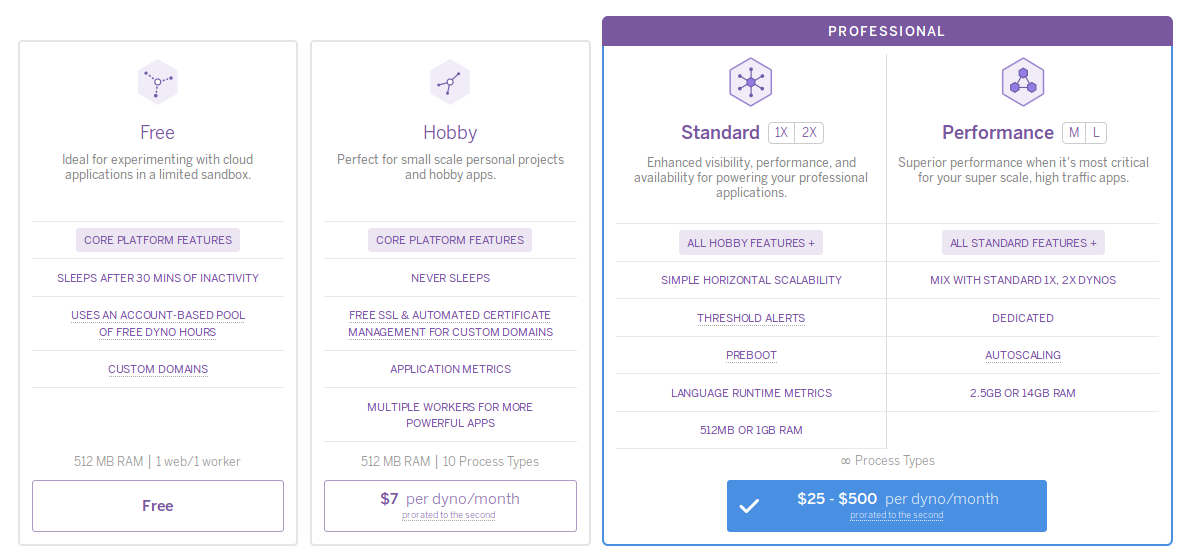
\includegraphics[width=\linewidth]{figuras/heroku-plan.png}
    \caption{Planes Heroku Cloud Platform}
    \label{fig::PlanesHerokuCloudPlatform}
\end{subfigure}

\begin{subfigure}{.6\textwidth}
    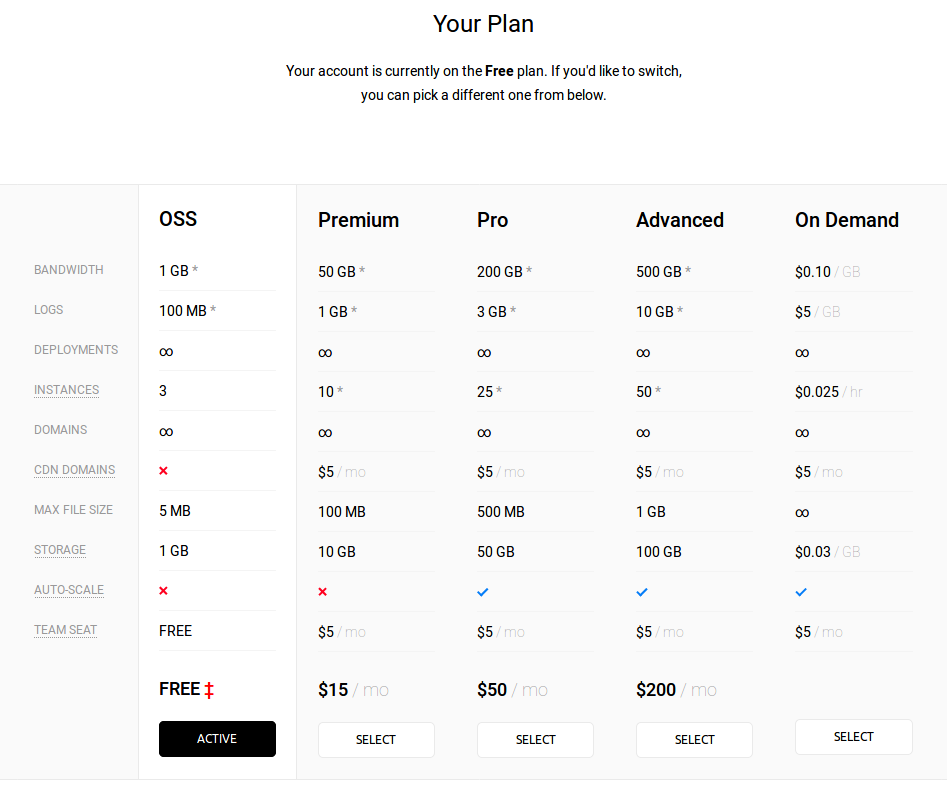
\includegraphics[width=\linewidth]{figuras/zeit-plan.png}
    \caption{Planes Zeit Platform}
    \label{fig::PlanesZeitPlatform}
\end{subfigure}

\begin{subfigure}{.6\textwidth}
    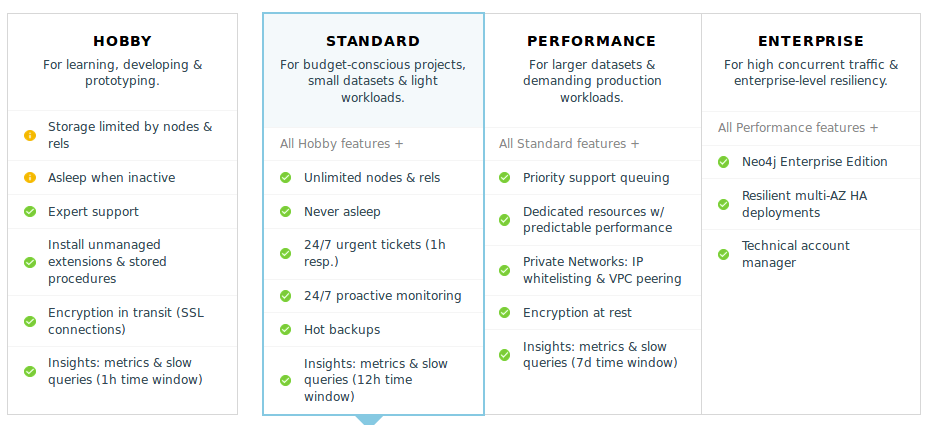
\includegraphics[width=\linewidth]{figuras/graphenedb-plan.png}
    \caption{Planes GrapheneDB Cloud} 
    \label{fig::PlanesGrapheneDBCloud}
\end{subfigure}
\caption{Planes \textit{cloud} de los distintos servicios del proyecto}
\label{fig::costes}
\end{figure}

\subsection{Coste total del proyecto}

En la tabla \ref{tab:: tablaCostes} se hace un resumen del coste total del proyecto.
	\begin{table}[htbp]
	\centering
	\begin{tabular}{|c|c|}
	\hline
	\textbf{Recurso}        & \textbf{Coste total } 	\\\hline
	Recursos   humanos  	& 10.400,59\euro             \\
	Recursos   materiales 	& 65,95\euro           		\\
	Costes   indirectos     & 400\euro      			    \\\hline 
	\textbf{Total}          & \textbf{	10866,54 \euro} \\     
	\hline
	\end{tabular}
	\caption{Tabla de costes del proyecto}
	\label{tab:: tablaCostes}
	\end{table}